\chapter{Firmware}
\label{ch:firmware}

\section{Análisis}
\label{sec:fw_analisis}

El primer paso para comenzar a trabajar en el firmware del dispositivo es realizar un análisis en el que se concreten los requisitos de las funcionalidades a incorporar al sistema.

Como se comentó en la sección \ref{sec:motivacion}, este proyecto es producto de las necesidades de Valeo, una empresa distribuidora de partes de vehículos. Junto a estas, pretenden también proporcionar a sus fabricantes herramientas para probar su correcto funcionamiento. Una de estas herramientas es el PWM Box.

En base a esto, se puede determinar que nuestro producto será usado principalmente en un entorno similar a una fábrica de coches o un taller mecánico. El perfil de su usuario principal será, por lo tanto, el de alguien que no necesariamente tenga conocimientos tecnológicos. Si se espera cierta familiaridad con dispositivos del entorno industrial, con controles similares al nuestro y una interfaz del mismo estilo.

Teniendo en cuenta las necesidades de la empresa y el perfil de este usuario, podemos definir los siguientes requisitos adicionales:

\clearpage

\subsubsection{Gestión de perfiles}

\begin{table}[h!]
    \centering
    \begin{tabular}{|m{2.5cm}|m{9.27cm}|}
        \hline
        \textbf{ID} & RF-1 \\
        \hline
        \textbf{Nombre} & Guardar perfiles \\
        \hline
        \textbf{Descripción} & El sistema debe permitir al usuario guardar la configuración activa en forma de perfil, que debe mantenerse en la memoria tras reiniciar el dispositivo. Esta operación debe estar protegida con contraseña, de forma que solo los usuarios autorizados puedan realizarla. \\
        \hline
        \textbf{Prioridad} & Alta \\
        \hline
    \end{tabular}
    \caption{RF-1. Guardar perfiles.}
\end{table}

\begin{table}[h!]
    \centering
    \begin{tabular}{|m{2.5cm}|m{9.27cm}|}
        \hline
        \textbf{ID} & RF-2 \\
        \hline
        \textbf{Nombre} & Cargar perfiles \\
        \hline
        \textbf{Descripción} & El sistema debe permitir al usuario cargar los perfiles almacenados en la memoria, estableciéndolos como activos. Esta operación debe estar protegida con contraseña, de forma que solo los usuarios autorizados puedan realizarla. \\
        \hline
        \textbf{Prioridad} & Alta \\
        \hline
    \end{tabular}
    \caption{RF-2. Cargar perfiles.}
\end{table}

\begin{table}[h!]
    \centering
    \begin{tabular}{|m{2.5cm}|m{9.27cm}|}
        \hline
        \textbf{ID} & RF-3 \\
        \hline
        \textbf{Nombre} & Eliminar perfiles \\
        \hline
        \textbf{Descripción} & El sistema debe permitir al usuario eliminar perfiles que estén actualmente almacenados en la memoria. Esta operación debe estar protegida con contraseña, de forma que solo los usuarios autorizados puedan realizarla. \\
        \hline
        \textbf{Prioridad} & Alta \\
        \hline
    \end{tabular}
    \caption{RF-3. Eliminar perfiles.}
\end{table}

\clearpage

\subsubsection{Gestión de la configuración del dispositivo}

\begin{table}[h!]
    \centering
    \begin{tabular}{|m{2.5cm}|m{9.27cm}|}
        \hline
        \textbf{ID} & RF-4 \\
        \hline
        \textbf{Nombre} & Guardar la contraseña \\
        \hline
        \textbf{Descripción} & El sistema debe almacenar la contraseña establecida en la memoria, de forma que esta se mantenga entre reinicios. \\
        \hline
        \textbf{Prioridad} & Alta \\
        \hline
    \end{tabular}
    \caption{RF-4. Guardar la contraseña.}
\end{table}

\begin{table}[h!]
    \centering
    \begin{tabular}{|m{2.5cm}|m{9.27cm}|}
        \hline
        \textbf{ID} & RF-5 \\
        \hline
        \textbf{Nombre} & Guardar el brillo de la pantalla \\
        \hline
        \textbf{Descripción} & Para la comodidad del usuario, el sistema debe almacenar la configuración de brillo del LCD en la memoria, de forma que esta se mantenga entre reinicios. \\
        \hline
        \textbf{Prioridad} & Media \\
        \hline
    \end{tabular}
    \caption{RF-5. Guardar el brillo de la pantalla.}
\end{table}

\subsubsection{Funcionalidad de señales lentas}

\begin{table}[h!]
    \centering
    \begin{tabular}{|m{2.5cm}|m{9.27cm}|}
        \hline
        \textbf{ID} & RF-6 \\
        \hline
        \textbf{Nombre} & Mostrar secuencias disponibles \\
        \hline
        \textbf{Descripción} & El sistema debe permitir al usuario consultar las secuencias lentas disponibles para ejecutar. Este menú debe ser independiente al resto del sistema. \\
        \hline
        \textbf{Prioridad} & Alta \\
        \hline
    \end{tabular}
    \caption{RF-6. Mostrar secuencias disponibles.}
\end{table}

\begin{table}[h!]
    \centering
    \begin{tabular}{|m{2.5cm}|m{9.27cm}|}
        \hline
        \textbf{ID} & RF-7 \\
        \hline
        \textbf{Nombre} & Ejecutar secuencias lentas \\
        \hline
        \textbf{Descripción} & El sistema debe permitir al usuario ejecutar las distintas secuencias lentas proporcionadas. \\
        \hline
        \textbf{Prioridad} & Alta \\
        \hline
    \end{tabular}
    \caption{RF-7. Ejecutar secuencias lentas.}
\end{table}

\begin{table}[h!]
    \centering
    \begin{tabular}{|m{2.5cm}|m{9.27cm}|}
        \hline
        \textbf{ID} & RF-8 \\
        \hline
        \textbf{Nombre} & Parar la ejecución de secuencias lentas \\
        \hline
        \textbf{Descripción} & El sistema debe permitir al usuario parar la ejecución de la secuencia activa en cualquier momento. \\
        \hline
        \textbf{Prioridad} & Alta \\
        \hline
    \end{tabular}
    \caption{RF-8. Parar la ejecución de secuencias lentas.}
\end{table}

\FloatBarrier

\subsubsection{Requisitos no funcionales}

\begin{table}[h!]
    \centering
    \begin{tabular}{|m{2.5cm}|m{9.27cm}|}
        \hline
        \textbf{ID} & RNF-1 \\
        \hline
        \textbf{Nombre} & Usabilidad \\
        \hline
        \textbf{Descripción} & El sistema ha de ser sencillo e intuitivo para los usuarios. \\
        \hline
        \textbf{Prioridad} & Alta \\
        \hline
    \end{tabular}
    \caption{RNF-1. Usabilidad.}
    \label{tab:rnf2}
\end{table}

\begin{table}[h!]
    \centering
    \begin{tabular}{|m{2.5cm}|m{9.27cm}|}
        \hline
        \textbf{ID} & RNF-2 \\
        \hline
        \textbf{Nombre} & Rendimiento \\
        \hline
        \textbf{Descripción} & El sistema debe ser fluido y responder a las acciones del usuario sin demoras. \\
        \hline
        \textbf{Prioridad} & Alta \\
        \hline
    \end{tabular}
    \caption{RNF-2. Rendimiento.}
\end{table}

\begin{table}[h!]
    \centering
    \begin{tabular}{|m{2.5cm}|m{9.27cm}|}
        \hline
        \textbf{ID} & RNF-3 \\
        \hline
        \textbf{Nombre} & Extensibilidad \\
        \hline
        \textbf{Descripción} & El sistema debe estar diseñado de forma que sea sencillo añadir nuevas características. \\
        \hline
        \textbf{Prioridad} & Media \\
        \hline
    \end{tabular}
    \caption{RNF-3. Extensibilidad.}
\end{table}

\section{Diseño}
\label{sec:fw_diseño}

Al tratarse de un desarrollo en proceso, el diseño de la arquitectura general del sistema ya estaba realizado. En este aspecto, los cambios a realizar son los derivados de la redistribución del código de algunas partes, que como se determinó en la sección \ref{sec:inginv}, dificultaba la incorporación de nuevas características.

\subsection{Menús}

El principal aspecto a rediseñar está en la parte del sistema que muestra los distintos menús al usuario. La idea es separar la actual implementación de los distintos menús en archivos independientes.

Por un lado, se creará un archivo de control, que será al que se haga referencia desde el resto del programa para hacer operaciones como cambiar de menú, actualizar la pantalla, cambiar el brillo del LCD, etc. Cuando se llamen a funciones que dependan de la pantalla que esté activa en ese momento, él será el que se encargue de delegar la tarea al menú que corresponda.

Por otro lado, cada menú disponible tendrá un archivo separado en el que se implementarán como mínimo las versiones correspondientes de las 3 operaciones básicas (actualizar pantalla, girar \textit{rotary encoder} y pulsar \textit{rotary encoder}). Esto permite que, en menús que requieran funciones específicas (como será el caso del menú de señales lentas que se pretende añadir), estas funciones sólo sean accesibles desde el menú que coresponda.

En la figura \ref{fig:fw_modules} incluída más adelante podemos ver el resultado de esta división. Se destaca también la inclusión de un nuevo tipo de menú, el menú del sistema. Este se encargará de mostrar la secuencia de inicio y el salvapantallas, tareas que estaban antes también unificadas con el resto. También será útil una vez se incluya el almacenamiento de perfiles en la memoria, pues permitirá mostrar un aviso cuando se llene la memoria.

\subsection{Entrada/Salida}

Para la parte de entrada/salida, también se entontraban agrupadas algunas funciones que no estaban del todo relacionadas entre sí. A la vez, se prevee necesario añadir nuevas funcionalidades relacionadas con la comunicación por el puerto serie para integrar el dispositivo con la interfaz gráfica, así como para solucionar los problemas detectados en el \textit{rotary encoder}.

Es por ello que se ha decidido dividir también el código de esta parte en 3 archivos: uno para el puerto serie, otro para el codificador rotarorio, y un tercero para el manejo de eventos.

\subsubsection{Especificaciones acerca de la comunicación por el puerto serie}

Para realizar la comunicación con la interfaz gráfica, se necesitará definir un formato para los mensajes que intercambie esta con el dispositivo.

En primer lugar, conviene determinar de alguna forma el comienzo y el final de un mensaje, lo que nos permitirá evitar errores procesando datos indebidos. Para el comienzo común servirá cualquier carácter que no se vaya a usar en ningún otro punto del mensaje. En este caso, se ha elegido el acento circunflejo (\verb|^|). Para el final, bastará con enviar un retorno de línea (\verb|\n|).

A continuación, se definirá un formato general para los mensajes. Como en este caso se va a realizar la comunicación por el puerto serie, que no es especialmente rápido, se priorizará que los mensajes sean lo más cortos posibles. De esta forma, llegamos a la siguiente especificación:

\begin{center}
    {\fontfamily{cmtt}\selectfont\verb|^T,C(,P1,P2 ... ,Pn)\n|}
\end{center}

Donde:

\begin{itemize}
    \item\textit{T} representa el tipo de mensaje, indicando \textit{?} una petición y \textit{!} un envío de datos.
    \item\textit{C} será una de las siguientes opciones, dependiendo del contenido que se esté transmitiendo:
        \begin{itemize}
            \item\textit{@} servirá como saludo inicial para establecer la conexión entre ambas partes.
            \item\textit{i} para información general del dispositivo.
            \item\textit{c} para la contraseña.
            \item\textit{n} se usará antes de enviar ranuras de memoria, para indicar cuántas.
            \item\textit{s} para ranuras (Slots) de memoria.
            \item\textit{p} para señales PWM.
        \end{itemize}
    \item\textit{Px} serán los distintos parámetros, que dependerán del comando enviado y se encuentran documentados en el código.
% TODO: ¿Añadirlos aquí?
\end{itemize}

Por último, cabría plantear el uso de algún mecanismo de detección de errores. En este caso, dada la baja complejidad y urgencia de la transmisión, se ha optado por posponer este aspecto del diseño, a la espera de probar la comunicación y determinar de forma experimental la frecuencia de errores.

\subsection{Memoria EEPROM}

Para el manejo de la memoria EEPROM, cabe especificar qué datos será necesarios guardar, así como la la forma en la que se van a almacenar los mismos.

En primer lugar se definirán las siguientes unidades:

\begin{itemize}
    \item\textbf{PWM:} Representación de una señal PWM en la memoria. Consistirá de sus 4 parámetros principales (modo, frecuencia, ciclo y fase), así como un nombre identificativo (por ejemplo, ``Intermitentes'').
    \item\textbf{Slot:} Llamado así por ser la unidad en la que se compartimentalizará la memoria (ranuras), representa una forma de agrupar señales PWM. Permitirá al usuario definir distintos modelos de coches de forma que cada PWM esté destinado a probar un grupo distinto de luces de faros. Consistirá de 8 señales PWM y de un nombre identificativo. Se añadirá, además, una variable que indicará si la ranura está ocupada o no. Esto permitirá evitar borrados reales de memoria, prolongando su vida útil y disminuyendo el coste en cuanto a rendimiento de la escritura.
\end{itemize}

Otros parámetros que se necesitarán guardar, teniendo en cuenta los requisitos establecidos son:

\begin{itemize}
    \item\textbf{Valor de inicialización:} Servirá para determinar si la memoria contiene o no datos, ya que en caso de que no los contenga, necesitará ser inicializada con algunos valores por defecto.
    \item\textbf{Número de serie:} Número identificador del dispositivo.
    \item\textbf{Versión del hardware}.
    \item\textbf{Versión del software}.
    \item\textbf{Brillo de la pantalla:} Permitirá mantener el brillo establecido entre ejecuciones.
    \item\textbf{Ranura por defecto:} Indica la ranura de memoria que se cargará automáticamente al iniciar el PWM Box.
    \item\textbf{Contraseña:} Debido al entorno en el que se plantea usar el dispositivo y al nivel de conocimiento técnico de sus usuarios, descrito en el anterior \hyperref[sec:fw_analisis]{análisis}, no se estima necesario encriptar la contraseña de ninguna forma.
\end{itemize}

Dada la capacidad del usuario de añadir, borrar y reemplazar ranuras de memoria según desee, se prevee la necesidad de algún mecanismo adicional para determinar qué ranuras mostrar en el menú principal del dispositivo. Con este fin, se incluirá también un vector auxiliar, que contendrá el índice de las ranuras de la memoria en el orden en el que se les muestra al usuario. Actúa, por así decirlo, como un traductor entre el índice de las ranuras visibles al usuario y el índice de las mismas internamente. Esto puede entenderse más fácilmente con una representación, que se incluye en la figura \ref{fig:eeprom_operations}

\begin{figure}[h!]
    \centering
    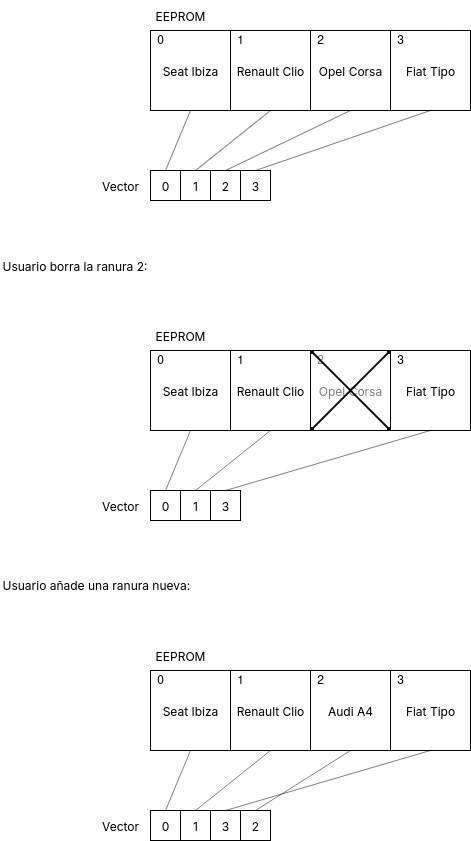
\includegraphics[width=0.8\textwidth]{eeprom_operations.png}
    \caption{Representación del funcionamiento del vector auxiliar al realizar distintas operaciones sobre la EEPROM.}
    \label{fig:eeprom_operations}
\end{figure}

\subsection{General}

La organización general de los archivos dentro del proyecto también se considera un aspecto importante a tener en cuenta para facilitar su manejo. Tras los cambios plantedos, algunos de los cuales incluyen la creación de aún más ficheros, esta necesidad se hace aún más aparente.

Para tratarlo, se plantea agruparlos en distintos directorios, a los que llamaremos módulos, de forma que queden distribuidos como se muestra en la figura \ref{fig:fw_modules}.

\begin{figure}[h!]
    \centering
	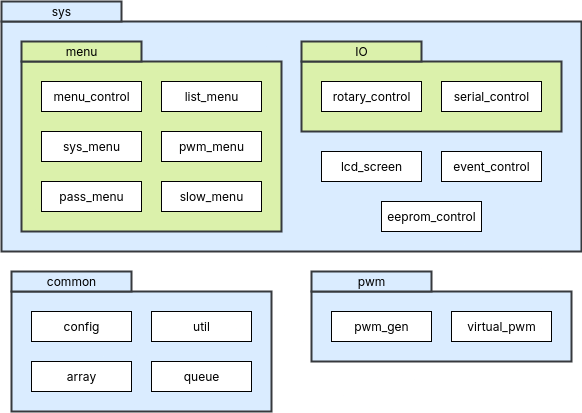
\includegraphics[width=\textwidth]{fw_modules.png}
	\caption{Distribución del código en distintos archivos y módulos.}
    \label{fig:fw_modules}
\end{figure}

\begin{itemize}
    \item\textbf{Módulo del sistema:} Contiene la implementación de características claves para el funcionamiento del sistema.
        \begin{itemize}
            \item\textbf{Módulo de E/S:} En él entontramos los archivos que definen el funcionamiento del \textit{rotary encoder} y de la UART, responsables de la comunicación con el usuario y la aplicación respectivamente.
            \item\textbf{Módulo de menús:} Agrupa la implementación de los distintos menús que usa el sistema.
        \end{itemize}
    \item\textbf{Módulo de PWM:} Se encarga de la generación y configuración de las señales de salida.
    \item\textbf{Módulo de archivos comunes:} Se tratan de utilidades genéricas, pensadas para ser usadas en común por las distintas partes del programa.
\end{itemize}

De esta forma, los distintos archivos quedan más agrupados según su funcionalidad, haciendo más viable establecer cierta encapsulación del código. Esto es especialmente importante teniendo en cuenta que el lenguaje con el que se trata no se especializa en la programación orientada a objetos, por lo que no permite definir clases al contrario que su sucesor. Podemos ver cómo quedaría la ejecución del bucle principal en la representación de la figura \ref{fig:fw_loop}. Adicionalmente, la figura \ref{fig:fw_interrupts} muestra el manejo de las interrupciones.

\begin{figure}[h!]
    \centering
    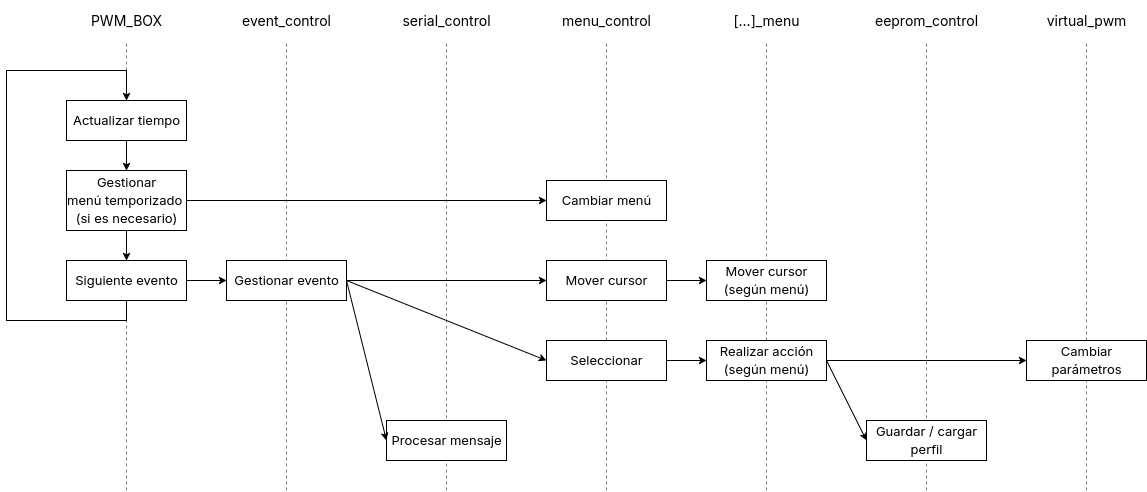
\includegraphics[width=\paperwidth,angle=-90,origin=c]{fw_loop.png}
    \caption{Ejecución del bucle principal.}
    \label{fig:fw_loop}
\end{figure}

\begin{figure}[h!]
    \centering
    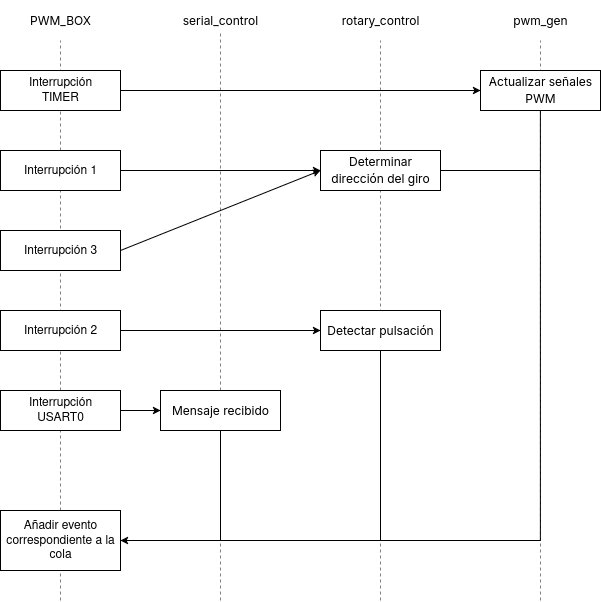
\includegraphics[width=\textwidth]{fw_interrupts.png}
    \caption{Ejecución de las distintas interrupciones.}
    \label{fig:fw_interrupts}
\end{figure}

\section{Desarrollo}

En esta sección se detallarán las decisiones enfrentadas durante la implementación del firmware, centrando la atención en los requerimientos definidos.

% Cabe destacar que también se ha realizado una extensa labor de limpieza del código, debido a una gran cantidad de declaraciones sin usar, definiciones redundantes y algunas prácticas que no se consideraban óptimas. En muchos casos, el código ha sido prácticamente reimplementando. Esto es, por supuesto, un aspecto subjetivo, por lo que no se hará referencia a ello nuevamente. Sin embargo, no mencionarlo sería subestimar el trabajo realizado en esta parte del proyecto.

Cabe mencionar, como regla general, que la mayoría sino todos los apartados incluidos en esta sección hacen uso de una forma u otra del \textit{datasheet} del ATmega 2560 \cite{atmega2560}, microcontrolador incluido en el Arduino Mega 2560 del que se hace uso en este proyecto.

\subsection{Menú de señales lentas}

La funcionalidad de este menú se basa en un contador ejecutado en el bucle principal, que se incrementa cada medio segundo. Este es el máximo común divisor de la frecuencia con la que se actualizan estas señales. Cuando el usuario escoge una secuencia, este contador comienza a incrementarse, y a compararse en cada unidad con los instantes en los que la señal debe cambiar, los cuales se encuentran definidos en un \textit{switch}. Esto permite cambiar la señal a una frecuencia menor de la que el dispositivo soporta de base, pudiendo realizar pruebas en faros que así lo requieran.

Para que este menú sea independiente del resto del sistema, se ha implementado en el \textit{rotary encoder} la capacidad de detectar cuándo el botón ha sido mantenido (más detalles en la siguiente subsección). Cuando esto ocurra, el sistema mostrará esta pantalla.

\subsection{\textit{Rotary encoder}}

En este ámbito, el objetivo principal era el de corregir el funcionamiento algo errático del \textit{rotary encoder}. Sin embargo, la lógica del código presente no estaba del todo clara, por lo que se acabó reimplementando desde cero. Esto también ha permitido incluir la posibilidad de detectar pulsaciones largas del botón, como se ha mencionado en el apartado anterior.

\subsubsection{Pulsaciones}

El pin correspondiente del microcontrolador está programado para generar una interrupción en cada cambio de flanco. Esto, en el caso del botón, quiere decir que se generará una interrupción al pulsarse el mismo y otra al soltarse. En cada una, habrá por lo tanto que comprobar el estado del botón en ese instante. En caso de que se encuentre pulsado, se guardará en una variable ese instante de tiempo. Si por el contrario no está pulsado, se comparará la variable anterior con el instante actual (momento en el que termina la pulsación). De esta forma, se determina si el botón se ha pulsado o si se ha mantenido. Este será el resultado de la operación, cuyo evento correspondiente se añadirá al buffer en la rutina de la interrupción.

A esto se le añade una pequeña lógica de \textit{debouncing}, que sólo tendrá en cuenta cada pulsación si la anterior se ha realizado fuera de una breve ventana de tiempo. Esto evita la detección de pulsaciones duplicadas debido a inexactitudes en el circuito del codificador.

\subsubsection{Giros}

La lógica para el giro del \textit{rotary encoder} es más compleja. Debido al funcionamiento del mismo, la dirección de giro se puede determinar según \textbf{el orden} en el que dos pines emitan voltaje. De esta forma, determinando la secuencia de estados por los que pasan los pines al realizar giros para las dos direcciones, se puede crear una máquina de estados. Esta, comprobando el estado actual de los pines al manejarse la interrupción, determinará cuándo se ha completado una rotación. Al igual que en el caso anterior, cuando esto ocurra, se incluirá el evento correspondiente en la cola de eventos, que será procesado por el sistema.

Para seguir este método, también se programa el microcontrolador para que emita una interrupción en ambos flancos de ambos pines, y se va comparando su estado con el de la máquina de estados mencionada. Este funcionamiento se ha encontrado en la librería \url{https://github.com/buxtronix/arduino/tree/master/libraries/Rotary}, cuyo código fuente ha sido adaptado para funcionar en este proyecto.

% Un rotary encoder consiste de un disco giratorio sobre el que se distribuyen unas zonas de contacto. El disco suele conectarse a tierra, mientras que las zonas de contacto servirán para transmitir voltaje. Al girar el rotary encoder, ambos pines A y B harán contacto con una de las zonas brevemente, generándose un pulso representable como una señal cuadrada.

\subsection{Serial control}

Una de los factores más importantes para la comunicación del puerto serie es configurar correctamente los puertos del microcontrolador. En este caso, se han habilitado las interrupciones RX (para la recepción) y TX (para el envío) y se ha configurado la comunicación para usar 8-bits por segmento.

Una de las desventajas de usar el puerto seria para la comunicación, es que sus velocidades de transmisión no son especialmente altas. Por ello, se plantea activar el modo \textit{Double Speed Operation} del ATmega 2560 para llegar a 115200 baudios. Con este, el valor a establecer en el puerto UBBR vendrá dado por la siguiente ecuación: \cite{atmega2560}

\begin{center}
    \[UBBR = \frac{f_{OSC}}{8 \cdot BAUD} - 1\]
\end{center}

Habiendo configurado el microcontrolador, el resto de la implementación se basa en definir funciones básicas que accedan al registro UDR0. Posteriormente, se usan estan funciones para implementar el sistema de envío y recepcion de datos, ya cubiertos en la \ref{sec:fw_diseño}.

\subsection{Memoria EEPROM}

Esta parte se ha implementado utilizado el apoyo de la librería \verb|avr/eeprom.h|, que proporciona la directiva \verb|EEMEM|, la cual permite declarar variables en la memoria EEPROM. Estas, sin embargo, solo sirven para poder hacer referencia a la dirección de memoria en la que se encuentran los datos desde el programa. Para leer su valor o escribir en ellas, es necesario usar las funciones proporcionadas por la misma librería. Por ello, la mayoría de funciones incluídas en esta parte no son más que distintos \textit{getters} y \textit{setters} para las distintas variables determinadas en la sección \ref{sec:fw_diseño}.

A estas se une el vector auxiliar tambien mencionado en la sección \ref{sec:fw_diseño}. Para facilitar su manejo y hacer el código más reutilizable, se ha implementado una pequeña librería que define las funciones básicas esperables de un vector.

Con todo esto, el contenido de la memoria EEPROM puede verse en la figura \ref{fig:eeprom_vars}.

\begin{figure}[h!]
    \centering
    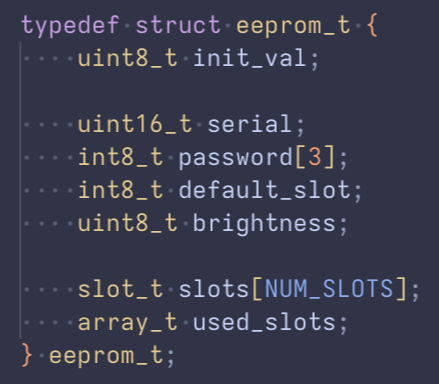
\includegraphics[width=0.5\textwidth]{eeprom_vars.png}
    \caption{Contenido de la memoria EEPROM.}
    \label{fig:eeprom_vars}
\end{figure}

Cuando, más adelante en el desarrollo, se comenzó a trabajar en la interfaz, se detectó un gran problema con el rendimiento a la hora de obtener los datos del dispositivo. El causante era que se estaban leyendo los datos directamente de la EEPROM siempre que la interfaz los pedía. Cada tiempo de acceso a un dato en memoria supone una gran penalización en el rendimiento del programa, que se hizo aparente incluso al leer únicamente la contraseña. Si se mantenía este funcionamiento, la calidad del producto final se vería muy perjudicada.

Es por ello que hubo que tomar la decisión de mantener en todo momento una copia de los datos de la EEPROM en la memoria del programa.

Por un lado, esto soluciona el problema comentado, ya que leer datos de la RAM es mucho más rápido que el caso anterior. Además, puede evitar escrituras innecesarias en la EEPROM, comparando el valor que se pretende guardar con el presente para detectar si realmente ha habido un cambio (también posible anteriormente, pero con la penalización del tiempo de acceso). Esto supone una mayor vida útil de la memoria programable.

Sin embargo, dado que la directiva \verb|EEMEM| ya reserva espacio para las variables en la memoria RAM, esto provoca en la práctica que las variables de la memoria EEPROM ocupen el doble de espacio. Dado que la memoria RAM del Arduino Mega 2560 tiene el doble de tamaño que su EEPROM, esto solo reduce en dos el número de perfiles que podemos almacenar, lo cual se considera un precio justo a pagar para cumplir el \hyperref[tab:rnf2]{RNF-2}.

\section{Pruebas}

Debido a la naturaleza del trabajo, la mayoría de pruebas se han realizado de manera experimental, observando los efectos de los cambios realizados sobre los distintos elementos.

Para comprobar que no se ha alterado la capacidad del dispositivo de emitir las señales de manera correcta, así como validar la implementación de las señales lentas, se ha usado un analizador lógico. En la figura \ref{fig:fw_pwm_signals} se muestran las señales PWM resultantes de distintas configuraciones. Adicionalmente, en las figuras \ref{fig:fw_slow_signal1} y \ref{fig:fw_slow_signal2}, se ven dos de las secuencias de señales lentas incluídas con el dispositivo.

\begin{figure}[h!]
    \centering
    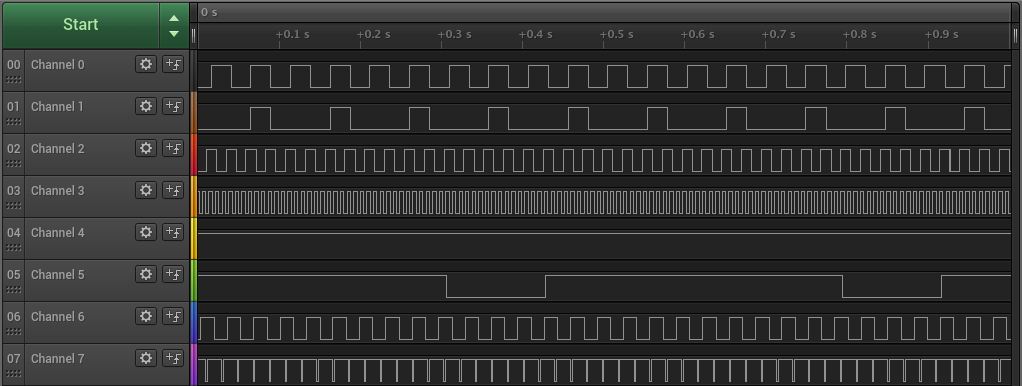
\includegraphics[width=\textwidth]{fw_pwm_signals.png}
    \caption{Señales PWM con distintas configuraciones.}
    \label{fig:fw_pwm_signals}
\end{figure}

\begin{figure}[h!]
    \centering
    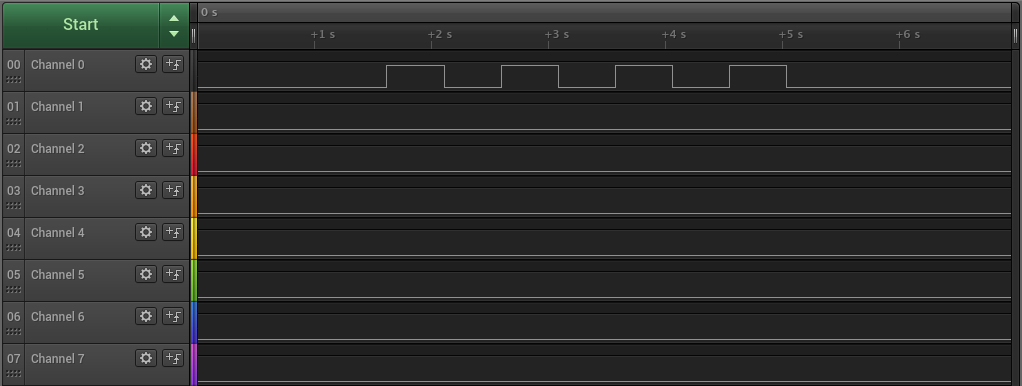
\includegraphics[width=\textwidth]{fw_slow_signal1.png}
    \caption{Una de las secuencias de señales lentas preconfiguradas.}
    \label{fig:fw_slow_signal1}
\end{figure}

\begin{figure}[h!]
    \centering
    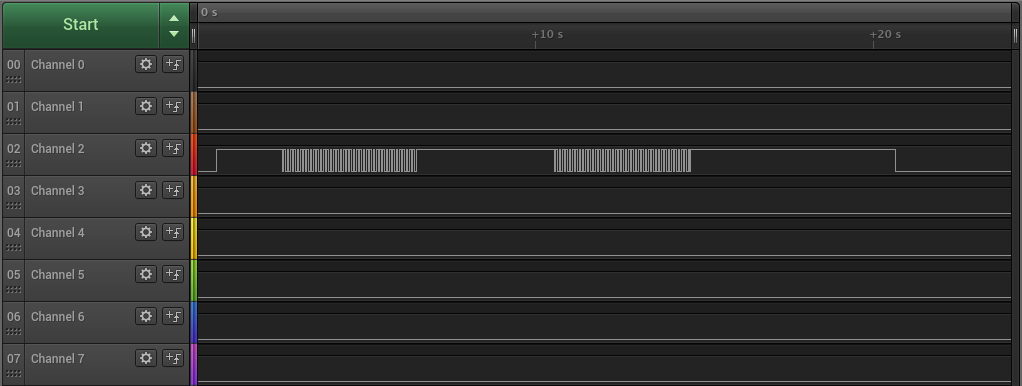
\includegraphics[width=\textwidth]{fw_slow_signal2.png}
    \caption{Otra de las secuencias de señales lentas preconfiguradas.}
    \label{fig:fw_slow_signal2}
\end{figure}

Estas pruebas han sido realizado con el Saleae Logic v1.2.40 \cite{saleae-logic}, que es \textit{software} propietario. Sin embargo, también podría usarse una versión \textit{open-source} como puede ser Sigrok PulseView v0.4.2 \cite{sigrok-pv}.
